\documentclass{report}
\usepackage[a4paper, total={7.5in, 10in}]{geometry}
\usepackage{polski}
\usepackage[utf8]{inputenc}
\usepackage{amsmath}
\usepackage{amssymb}
\usepackage{graphicx}
\usepackage{float}
\usepackage{amsfonts}
\usepackage{sectsty}
\usepackage{titlesec}
\usepackage{setspace}
\usepackage{booktabs}
\usepackage{stix}
\usepackage{fancyhdr}
\usepackage{hyperref}
\usepackage{caption}

\usepackage{enumitem}
\usepackage{pgfplots}
\usepackage{etoolbox}
\usepackage{subcaption}
\usepackage{multirow}
\usepackage{xcolor}
\usepackage{enumitem}
\graphicspath{ {zdj} }
\pagestyle{empty}

\setlength{\parindent}{0pt}

\newcommand\setItemnumber[1]{\setcounter{enumi}{\numexpr#1-1\relax}}



\titlespacing*{\chapter}{0pt}{-35pt}{0pt}
\titlespacing*{\section}{0pt}{-20pt}{10pt}
\titlespacing*{\subsection}{0pt}{-20pt}{10pt}
\titlespacing*{\subsubsection}{0pt}{0pt}{10pt}

\titleformat{\chapter}[display]{\normalfont\Large\bfseries\filcenter}{}{10pt}{\Large}
\titleformat{\section}[display]{\normalfont\large\bfseries\filcenter}{}{10pt}{\large}
\titleformat{\subsection}[display]{\normalfont\normalsize\bfseries\filcenter}{}{10pt}{\normalsize}
\titleformat{\subsubsection}[display]{\normalfont\small\bfseries}{}{10pt}{\small}

\setcounter{tocdepth}{3}
\setcounter{secnumdepth}{3}

\pagestyle{fancy}
\fancyhf{}
\fancyfoot[R]{Strona \thepage}
\renewcommand{\headrulewidth}{1pt}
\renewcommand{\footrulewidth}{1pt}
\fancypagestyle{plain}{\pagestyle{fancy}}

\fancyfoot[L]{Popławski Dawid}%
\fancyhead[R]{}%


\DeclareCaptionFormat{custom}
{%
	\textbf{#1#2}\textit{\small #3}
}
\renewcommand{\figurename}{Rys.}

\captionsetup{format=custom,%
				margin={5pt,5pt},%
				justification=centering}
\usepackage[T1]{fontenc}       % change font encoding to T1
\usepackage[framed,numbered]{matlab-prettifier}



\begin{document}
	\begin{titlepage}
		\begin{figure}[h]
			\begin{minipage}[l]{.5\textwidth}%
				
\includegraphics[width=0.3\textwidth]{pwr_logo}
			\end{minipage}%
			\begin{minipage}[r]{.5\textwidth}%
				
\includegraphics[width=1\textwidth]{wit_logo}
			\end{minipage}%
		\end{figure}
		
		\vspace*{3mm}
		
		\begin{center}
			\rule{\textwidth}{0.8pt}\\ 
			\vspace*{6mm}
			{\LARGE Platformy programistyczne .Net i Java - LAB1-2}\\
			\vspace*{3mm}
			\rule{\textwidth}{0.8pt}\\
			
			\vspace{1.5cm}
			{\setstretch{2}
				Politechnika Wrocławska
				
				Wydział Informatyki i telekomunikacji
				
				Kierunek: Informatyczne systemy automatyki
				
				grupa nr 2
				
				\href{https://github.com/wernexnrs/264254-.NET-i-Java}{github.com/wernexnrs/264254-.NET-i-Java}
				
			}
		\end{center}
		
		\vspace*{2cm}
		
		\begin{flushright}
			{\setstretch{2}
				Dawid Popławski - $264254$
				
				Termin zajęc: Środa godz. $17^{\underline{05}}$ - $18^{\underline{45}}$ 
				
				Prowadzący: mgr inż. Michał Jaroszczuk
				
			}
			
		\end{flushright}
		
		\vfill
		
\end{titlepage}

\tableofcontents

\chapter{Opis problemu}

\vspace{5pt}
Problem plecakowy to klasyczny problem optymalizacyjny, który polega na wybraniu zestawu przedmiotów o maksymalnej wartości, tak aby suma ich wag nie przekraczała określonej pojemności plecaka.\\

Dla każdego przedmiotu należało określić wartość binarną $x_i \in {0,1}$, gdzie "0" oznaczało, że przedmiot nie zmieścił się do plecaka. Pojemność plecaka jest ograniczona pewną ustaloną na początku wartością, gdzie:

\[
	\sum_{i=1}^{n}x_iw_i \leq C
\]
Zadaniem optymalizacyjnym było:

\[
	max\sum_{i=1}^{n}x_iv_i, \hspace*{15pt}\text{gdzie } v_i \text{--} \text{wartość, } w_i \text{--} \text{waga}
\]
Na potrzeby projektu należało założyć, że wartość i waga pojedyńczego przedmiotu będzie mieścić się w zakresie $v_i,w_i \in <1,10>$

\chapter{Aplikacja konsolowa}

\section{Drzewo projektu}

\begin{figure}[H]%
	\centering
	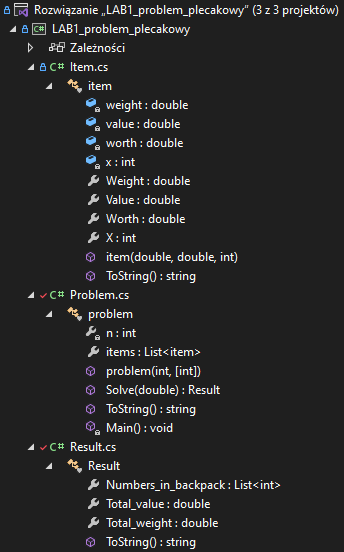
\includegraphics[scale=0.6]{zdj/cmd_drzewo}
	\caption{Drzewo projektu aplikacji konsolowej.}
\end{figure}

\section{Problem.cs}

W tym pliku definiujemy klasę problem, która reprezentuje i rozwiązuję problem plecakowy.

\begin{figure}[H]%
	\centering
	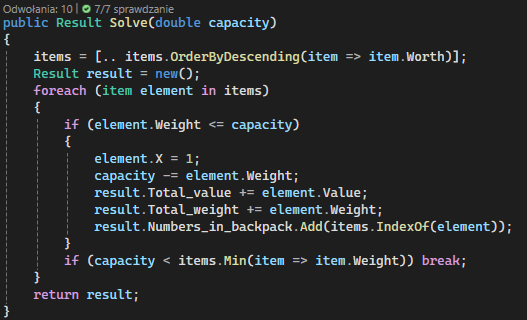
\includegraphics[scale=0.6]{zdj/algorytm_zachlanny}
	\caption{Kod rozwiązujący problem plecakowy.}
\end{figure}

Główny algorytm iteruje po wszystkich elementach listy i sprawdza, czy waga danego przedmiotu jest mniejsza bądź równa aktualnej pojemności plecaka. W przypadku spełnienia warunku pole "X" tego obiektu zmieniane jest na 1, od pojemności plecaka odejmowana zostaje waga wrzuconego przedmiotu oraz zliczania jest suma całkowitej wartości, całkowitej wagi, do tego zapisywany jest indeks przedmiotu i wstawiany do osobnej listy.


\chapter{Testy jednostkowe}

\section{Drzewo projektu}

\begin{figure}[H]%
	\begin{minipage}{0.5\linewidth}
		\centering
		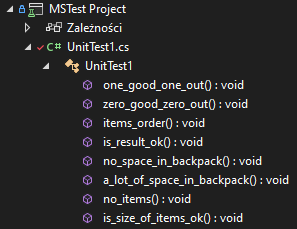
\includegraphics[scale=0.7]{zdj/testy_drzewo}
		\caption{Drzewo projektu testów jednostkowych.}
	\end{minipage}
	\begin{minipage}{0.5\linewidth}
		\centering
		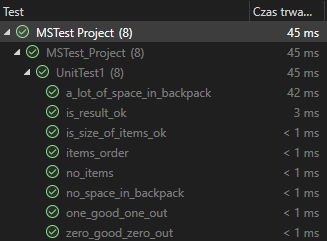
\includegraphics[scale=0.7]{zdj/test_result}
		\caption{Wynik testów jednostkowych.}
	\end{minipage}
\end{figure}


Zrealizowanie testy jednostkowe:

\begin{itemize}
	\item Sprawdzenie, czy jeśli co najmniej jeden przedmiot spełnia ograniczenia, to zwrócono co najmniej jeden element.
	\item Sprawdzenie, czy jeśli żaden przedmiot nie spełnia ograniczeń, to zwrócono puste rozwiązanie.
	\item Sprawdzenie, czy kolejność przedmiotów ma wpływa na znalezione rozwiązanie.
	\item Sprawdzenie poprawności wyniku dla konkretnej instancji.
	\item Sprawdzenie, czy jeżeli plecak nie ma miejsca to nie będzie w nim przedmiotów.
	\item Sprawdzenie, czy jeżeli plecak ma bardzo dużo miejsca to wszystkie przedmioty do niego trafiły.
	\item Sprawdzenie, czy algorytm działa gdy nie ma żadnych przedmiotów.
	\item Sprawdzenie, czy ilość wylosowanych przedmiotów zgadza się z ilością obiektów w liście.
\end{itemize}

\begin{figure}[H]%
	\centering
	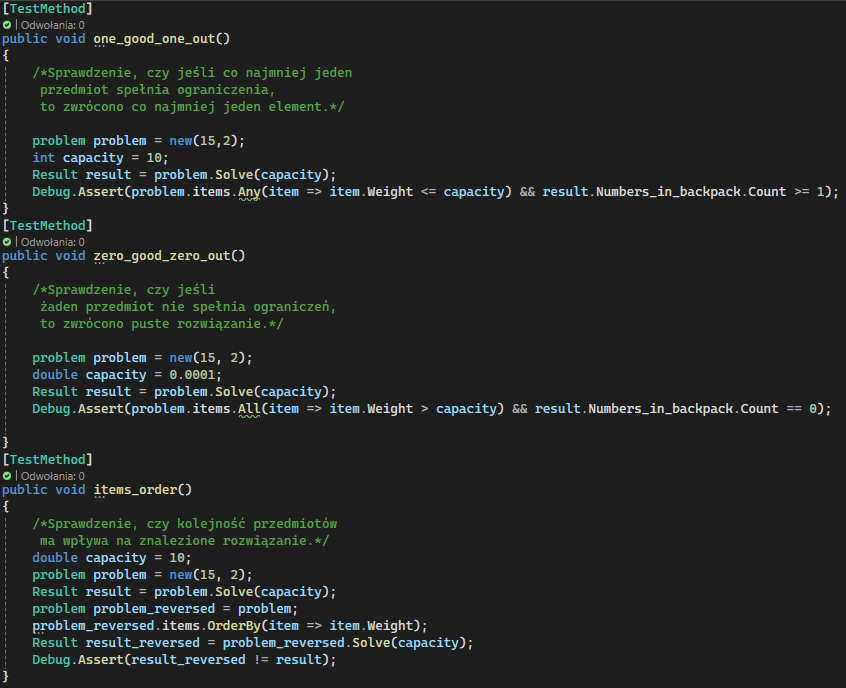
\includegraphics[scale=0.5]{zdj/test_first}
	\caption{Testy jednostkowe.}
\end{figure}

\begin{figure}[H]%
	\centering
	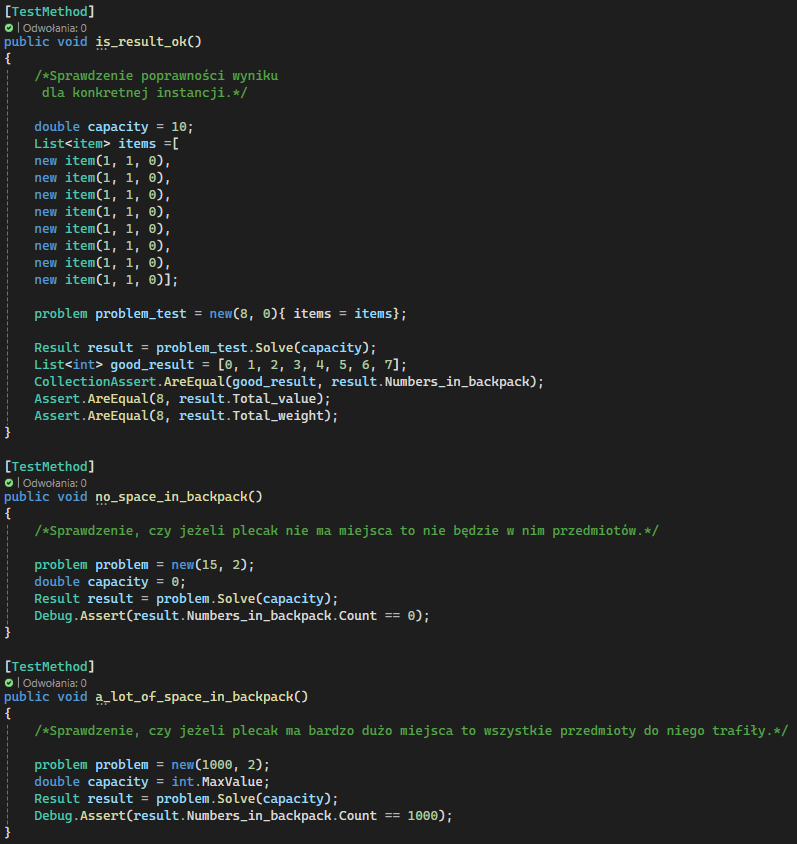
\includegraphics[scale=0.5]{zdj/test_second}
	\caption{Testy jednostkowe.}
\end{figure}

\begin{figure}[H]%
	\centering
	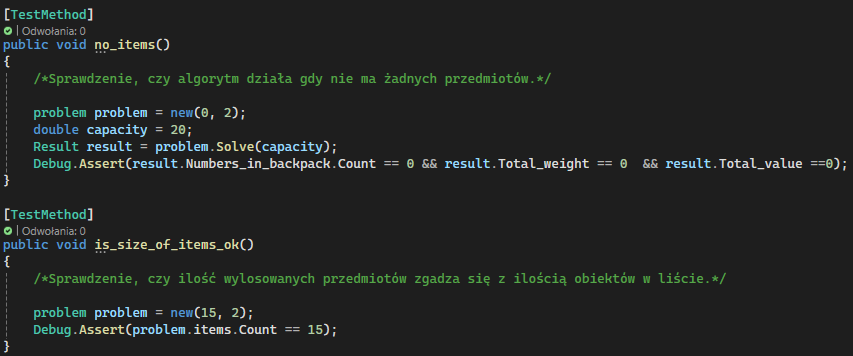
\includegraphics[scale=0.6]{zdj/test_third}
	\caption{Testy jednostkowe.}
\end{figure}

\chapter{Aplikacja okienkowa}

Aplikacja posiada proste zabezpieczenie w przypadku wpisania do texboxa innej wartości niż liczby. 

\section{Drzewo projektu}

\begin{figure}[H]%
	\centering
	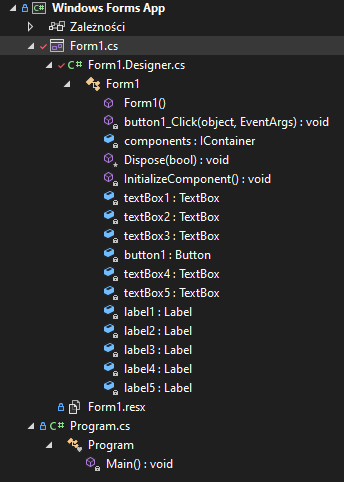
\includegraphics[scale=0.6]{zdj/form_drzewo}
	\caption{Drzewo projektu aplikacji okienkowej.}
\end{figure}


\begin{figure}[H]%
	\centering
	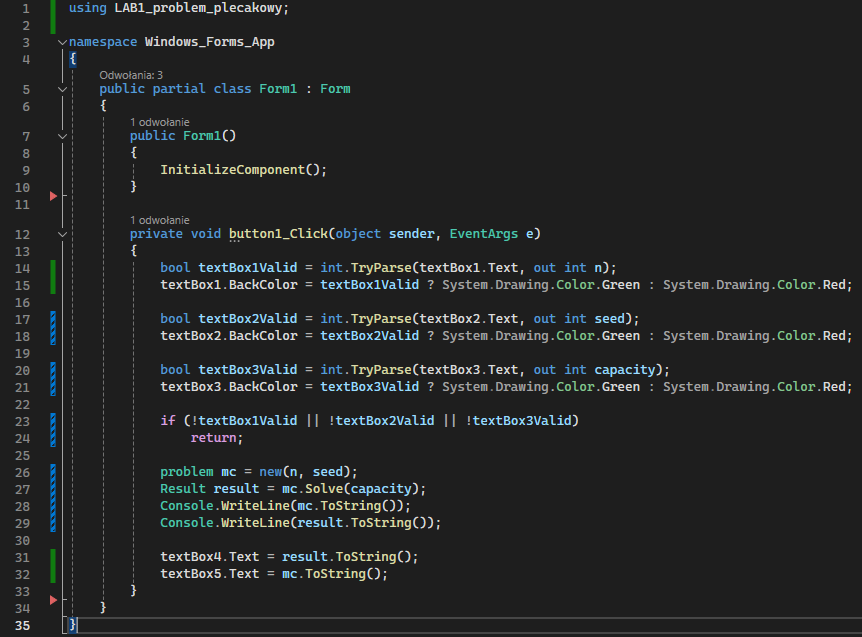
\includegraphics[scale=0.6]{zdj/form_code}
	\caption{Kod aplikacji okienkowej.}
\end{figure}


\end{document}